\documentclass{article}

\usepackage{graphicx}
\usepackage{tikz}
\usepackage{tikzsymbols}
\usetikzlibrary{calc,patterns,shapes.geometric}
\pagestyle{empty}
\usepackage[margin=0pt]{geometry}
\geometry{papersize={14in,12in}}

\def\centerarc[#1](#2)(#3:#4:#5){\draw[#1] ($(#2)+({#5*cos(#3)},{#5*sin(#3)})$) arc (#3:#4:#5);}

\begin{document}
	\begin{figure}
		\centering
		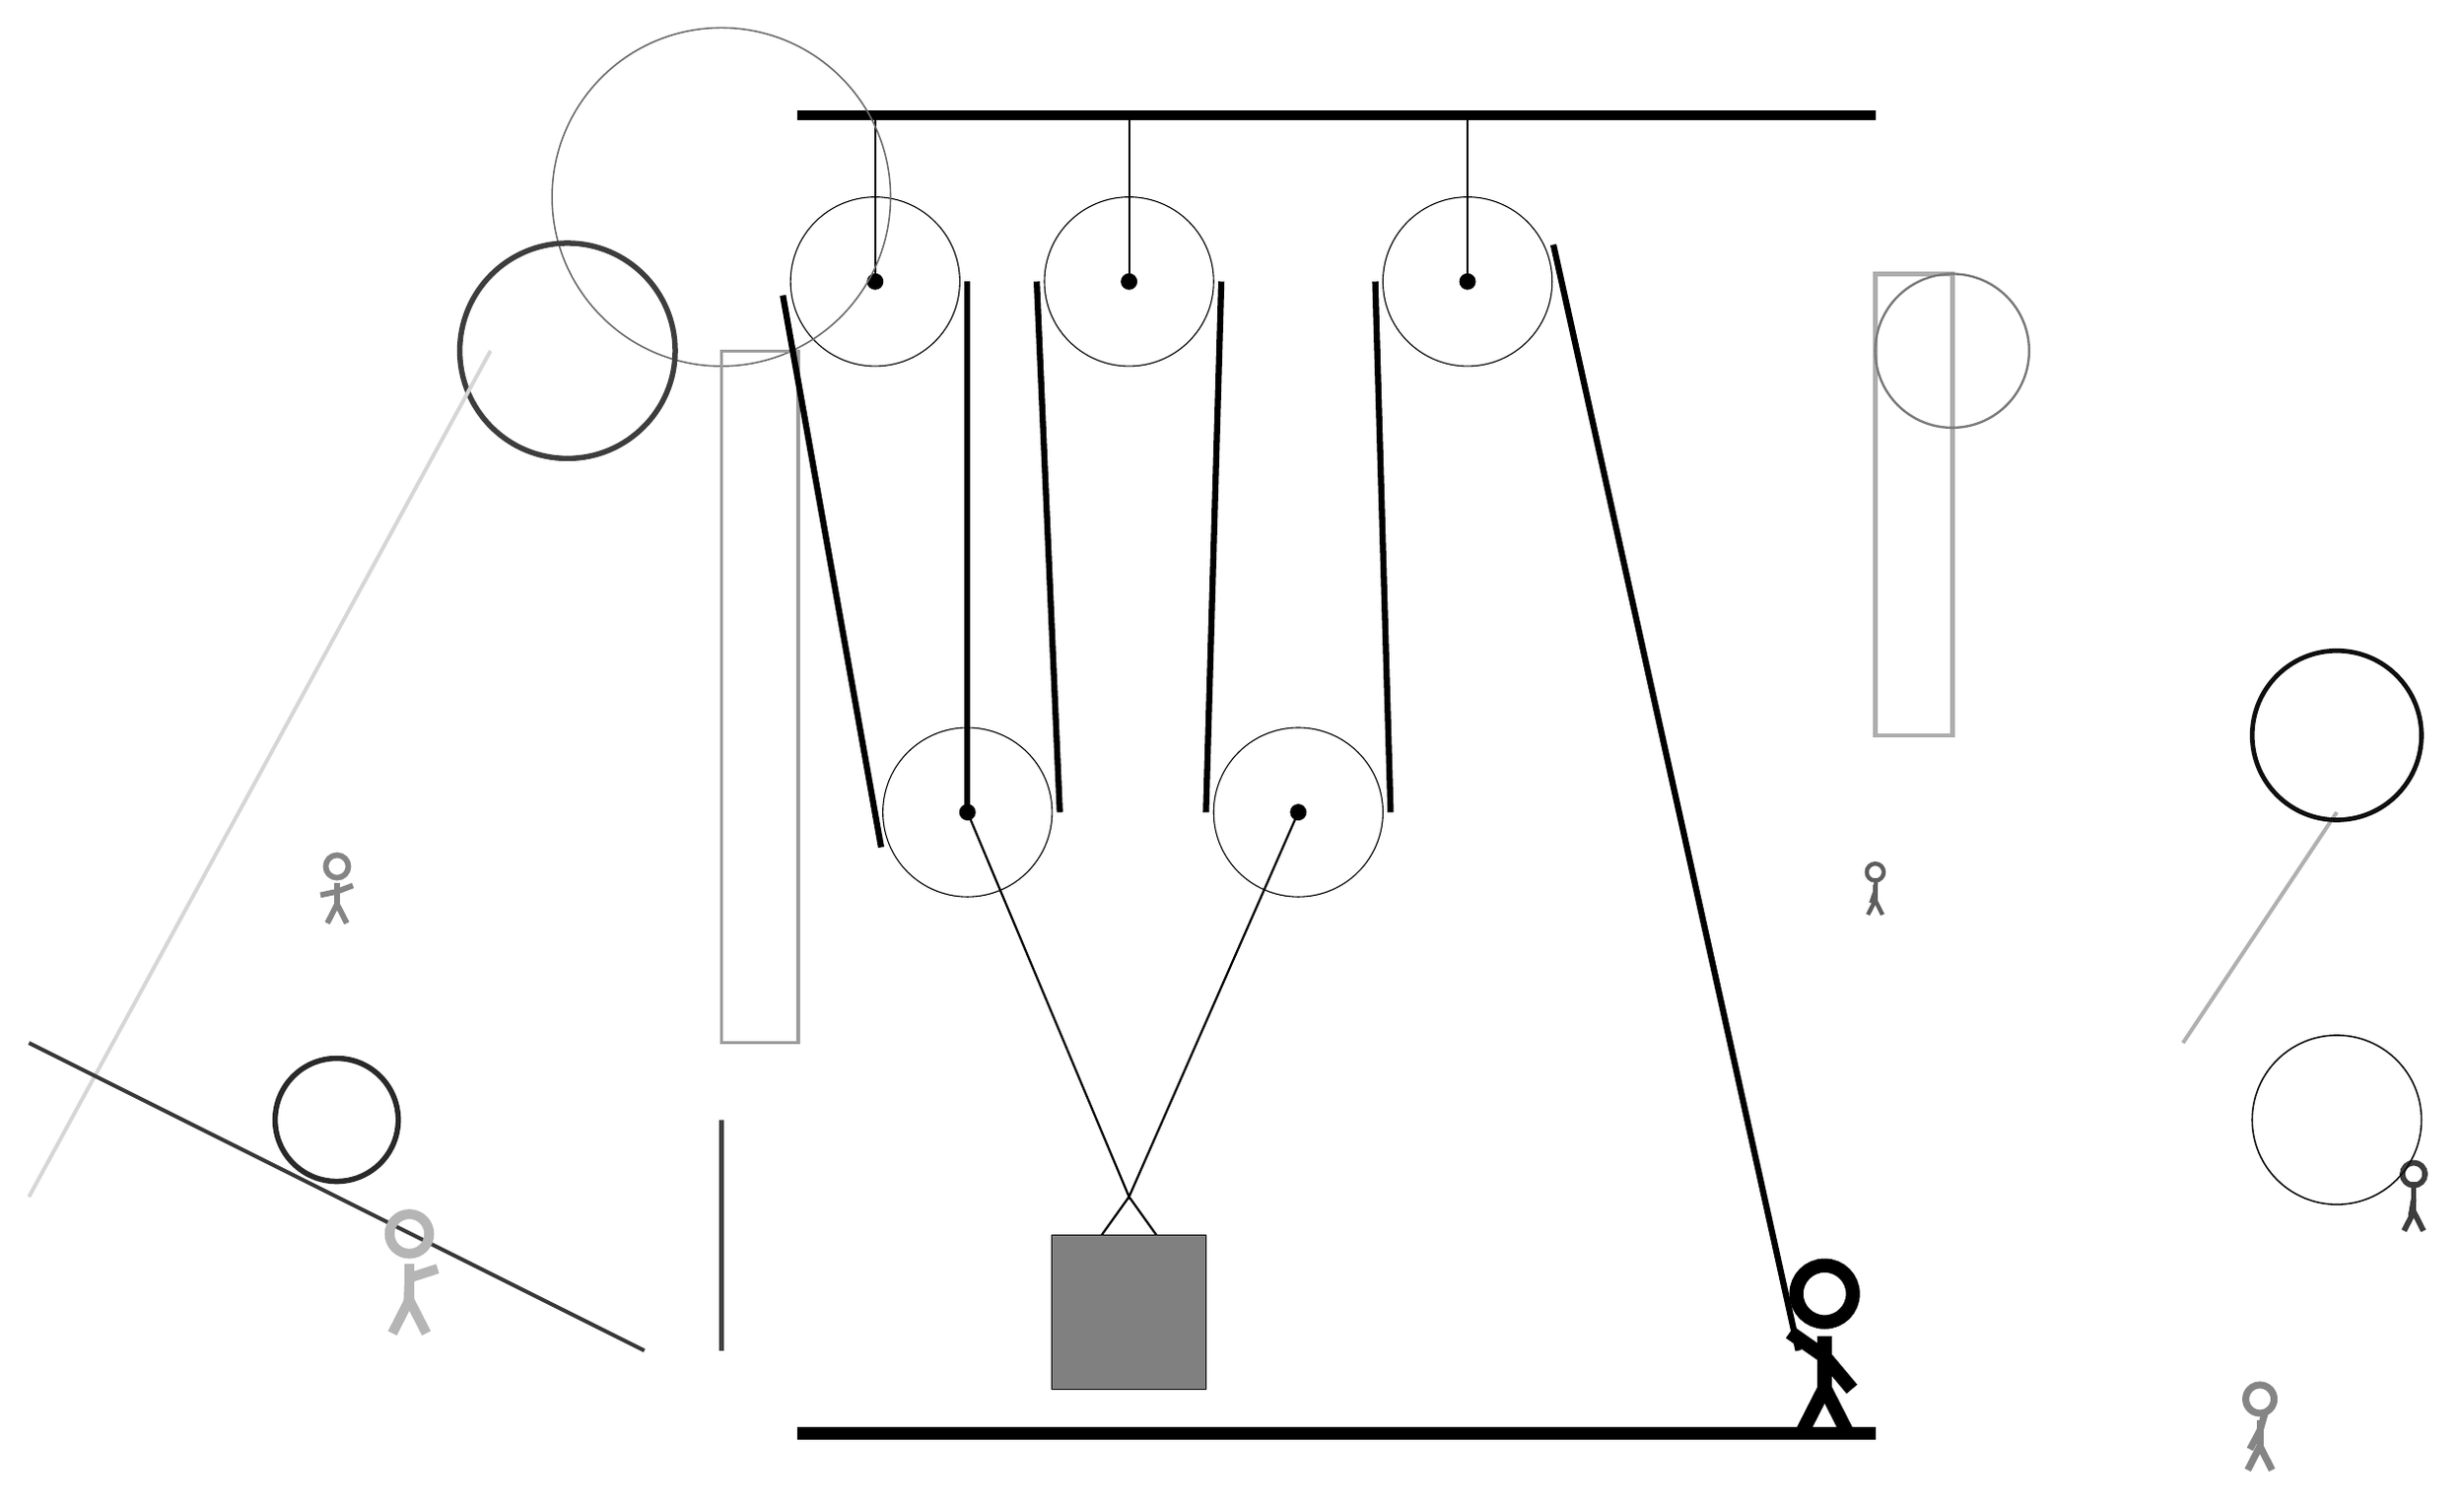
\begin{tikzpicture}
			%%%%% START %%%%%
			
			\draw[fill=black] (-2, 14) rectangle (12, 14.125);
			
			\draw (-1, 11.9) circle (1.1);
			\draw[fill=black] (-1, 11.9) circle (0.1);
			\draw[thick] (-1, 11.9) -- (-1, 14);
			
			\draw (2.3, 11.9) circle (1.1);
			\draw[fill=black] (2.3, 11.9) circle (0.1);
			\draw[thick] (2.3, 11.9) -- (2.3, 14);
			
			\draw (6.7, 11.9) circle (1.1);
			\draw[fill=black] (6.7, 11.9) circle (0.1);
			\draw[thick] (6.7, 11.9) -- (6.7, 14);
			
			\draw (0.2, 5) circle (1.1);
			\draw[fill=black] (0.2, 5) circle (0.1);
			
			\node[line width=0.2mm, color=black!48] at (-8, 4) {\Strichmaxerl[4][12][21]};
			
			\draw [line width=0.2mm, color=black!58](-3, 13) circle (2.2);
			\node[line width=0.2mm, color=black!63] at (12, 4) {\Strichmaxerl[3][71][86]};
			\draw [line width=0.7mm, color=black!76](-5, 11) circle (1.4);
			
			\draw[line width=0.5mm, color=black!31](16, 2) -- (18, 5);
			\draw[line width=0.5mm, color=black!16](-6, 11) -- (-12, 0);
			
			\draw[line width=0.6mm, color=black!74] (-3, 1) rectangle (-3, -2);
			\draw[line width=0.4mm, color=black!39] (-3, 2) rectangle (-2, 11);
			\node[line width=0.4mm, color=black!76] at (19, 0) {\Strichmaxerl[4][80][90]};
			
			\draw [line width=0.6mm, color=black!94](18, 6) circle (1.1);
			\draw[line width=0.5mm, color=black!78](-4, -2) -- (-12, 2);
			\draw [line width=0.7mm, color=black!84](-8, 1) circle (0.8);
			\draw [line width=0.2mm, color=black!95](18, 1) circle (1.1);
			
			\draw[line width=0.6mm, color=black!32] (13, 6) rectangle (12, 12);
			\node[line width=0.7mm, color=black!29] at (-7, -1) {\Strichmaxerl[7][88][18]};
			\node[line width=0.7mm, color=black!48] at (17, -3) {\Strichmaxerl[5][62][74]};
			
			\draw [line width=0.3mm, color=black!53](13, 11) circle (1.0);
			
			
			\draw (4.5, 5) circle (1.1);
			\draw[fill=black] (4.5, 5) circle (0.1);
			
			\draw[thick] (0.2, 5) -- (2.3, 0)  -- (4.5, 5);
			\draw[thick]  (1.8, -0.7) -- (2.3, 0) -- (2.8, -0.7);
			\draw[fill=black!50] (1.3, -0.5) rectangle (3.3, -2.5);
			
			\draw[line width=0.8mm] (0.2, 5) -- (0.2, 11.9);
			\centerarc[line width=0.8mm](-1, 11.9)(0:200:1.2000000000000002);
			\draw[line width=0.8mm] (-2.2, 11.72) -- (-0.922, 4.544);
			\centerarc[line width=0.8mm](0.2, 5)(200:360:1.2000000000000002);
			\draw[line width=0.8mm](1.4, 5) -- (1.1, 11.9);
			\centerarc[line width=0.8mm](2.3, 11.9)(0:180:1.2000000000000002);
			\draw[line width=0.8mm] (3.5, 11.9) -- (3.3, 5);
			\centerarc[line width=0.8mm](4.5, 5)(180:360:1.2000000000000002);
			\draw[line width=0.8mm] (5.7, 5) -- (5.5, 11.9);
			\centerarc[line width=0.8mm](6.7, 11.9)(20:180:1.2000000000000002);
			\draw[line width=0.8mm](7.816, 12.38)  -- (11, -2);
			
			\node at (11.3, -2) {\Strichmaxerl[10][-35][-50]};
			
			\draw[fill=black] (-2, -3) rectangle (12, -3.15);
			
			%%%%% END %%%%%
		\end{tikzpicture}
	\end{figure}	
\end{document}